% \begin{savequote}[8cm]
% \textlatin{Neque porro quisquam est qui dolorem ipsum quia dolor sit amet, consectetur, adipisci velit...}

% There is no one who loves pain itself, who seeks after it and wants to have it, simply because it is pain...
%   \qauthor{--- Cicero's \textit{de Finibus Bonorum et Malorum}}
% \end{savequote}

\chapter{\label{ch:4-dents}Monte Carlo Tree Search With Boltzmann Exploration} 

    \minitoc

    This chapter discusses MCTS algorithms for planning in single-objective environments whose search policies take the form of Boltzmann distributions. Primarily, this chapter aims to answer question \entropyq, while laying the foundation to answer \contextq\ewe in Chapter \ref{ch:6-simplexmaps}.
    
    \begin{figure}
        \centering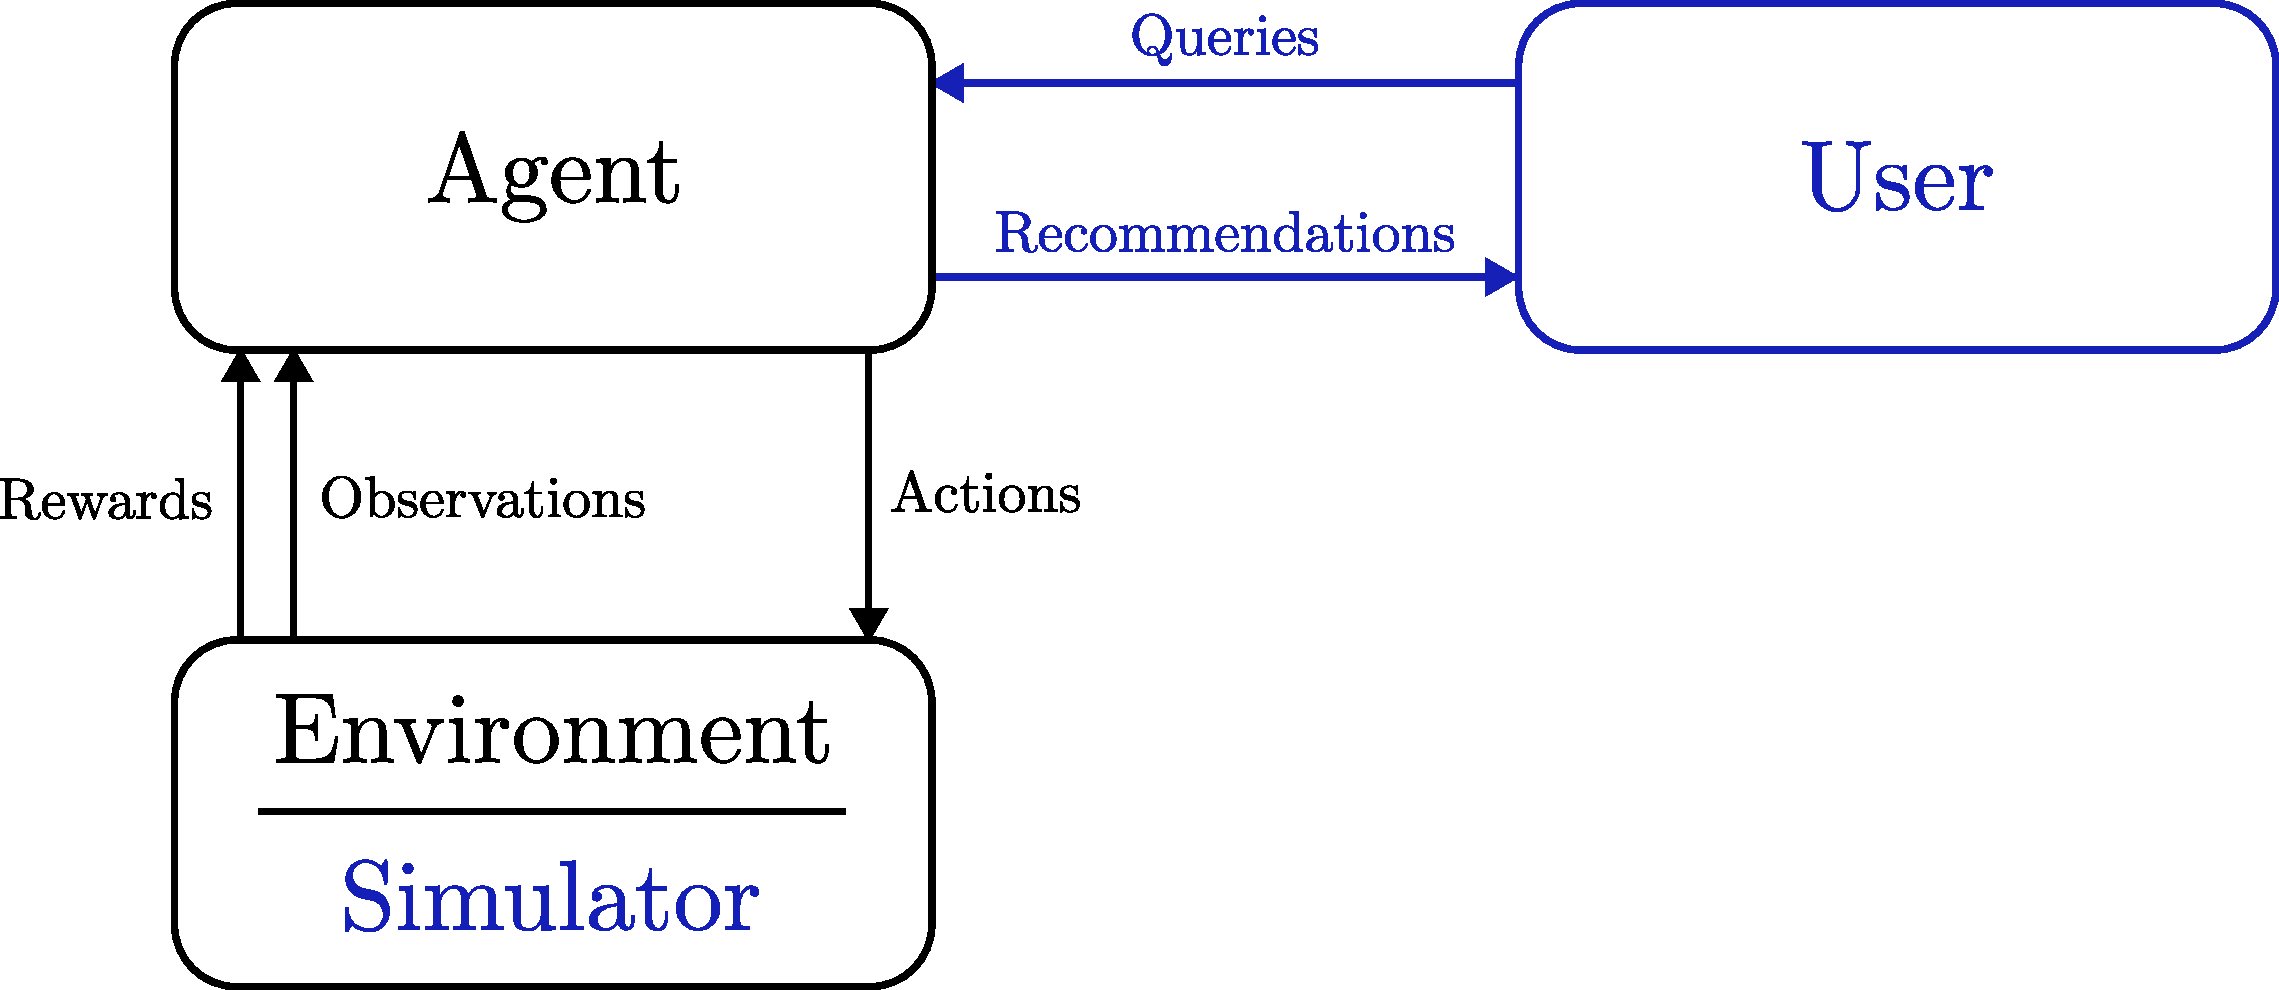
\includegraphics[width=0.75\textwidth]{figures/ch2/rl_overview.pdf} 
        \caption[Exploration setting in reinforcement learning.]{\todo{update fig to just be the blue version.} Exploration setting in reinforcement learning (\todo{reproduced and edited from fig 2.5}), \bd{where the agent aims to discover the optimal policy and has a larger emphasis on exploration to find better solutions rather than exploiting.}}
        \label{fig:4:rl_overview}
    \end{figure}

    Figure \ref{fig:4:rl_overview} gives the exploration setting for reinforcement learning, where the agent is only assessed on the recommendations that it provides, and is not penalised for considering poor actions in the simulator. 

    This chapter will also consider how entropuy can be used as an auxilary secondary objective to encourage exploration. Entropy is already used widely in the reinforcement literature \todo{cites, ppo, sac etc, ref ch3}, and is often cited for its \bd{exploration, and robustness to uncertainty, and robustness to simulator/environment differences, and robustness to noise.} 

    When considering the maximum entropy reinforcement learning objective (\todo{ref}), the optimal policy (equation (\todo{ref})) naturally takes the form of a Boltzmann policy. Notably, MENTS (Section \ref{sec:2-4-3-ments}), and RENTS and TENTS (Section \todo{ref litrev}) are existing MCTS algorithms for the maximum entropy setting (Section \ref{sec:2-3-1-merl}), so will be discussed further in this chapter, along with UCT (Section \todo{ref}), and used as baseline algorithms.

    Section \ref{sec:4-1-intro} discusses limitations of existing MCTS algorithms in this exploration setting, motivating the work covered in the remainder of the chapter. Additionally, the planning framework is defined so that the algorithms can be theoretically analysed using \textit{simple regret}.
    
    In Section \ref{sec:4-2-boltzmannsearch} the \textit{Boltzmann Tree Search} and \textit{Decaying ENtropy Tree Search} algorithms are defined.

    Section \ref{sec:4-3-toyenvs} considers some theoretical MDPs, which are used to empirically demonstrate the limitations of the existing MCTS algorithms, and are used for constructive proofs of some theorems. 

    Results on grid world and the game of Go are given in section \ref{sec:4-4-results}. 

    Finally, in Section \ref{sec:4-5-theory} the main theoretical analysis and proofs are given.

    \todo{add sect 4.6 if actually use that.}

    \todo{one paragraph for ch overview? Or make other descriptions longer? Or make it bullet points?}

    \todo{After finished writing, do another pass through neurips paper and check no results/writing missing from thesis that really should be included. (Thinking about some of the frozen lake plots in the appendix when writing this.)}
    







\section{Introduction and Motivation}
\label{sec:4-1-intro}

    UCT \todo{ref} \bd{is designed in the traditional reinforcement learning setting (todo ref Fig 2.5), minimising the cumulative regret (todo ref)}, and so UCT makes a trade off between exploration and exploitation. As such, UCT will frequently choose the same action to exploit, which results in it getting stuck in local optima when \bd{rewards are sparse or not informative.}

    To see this consider two grid world MDPs which differ only in the reward function. \todo{state space is (x,y,time), actions are cardinal directions etc}. The first reward function is to use a constant cost of $R_1(s,a)=-1$, and the second is a sparse version where the time cost is only revealed at the end $R_2((x,y,t),(x_a,y_a)) = -(t+1)\one[(x,y)+(x_a,y_a)==G]$. \todo{clean and actually define goal state, and name bettwer than R1 and R2}

    \todo{make diagram}

    \todo{something that says although this example can be solved by using the more sensible reward, it's just to highlight the issue of exploration}.
    
    \todo{would like to have figs showing the best path found by UCT in both cases AND showing the number of trials (one step of branches) where it explored.}

    Although the issues in the above toy problem can be resolved by using the simpler constant reward $R_1$, the example serves to highlight that UCT performs best when provided with a dense and informative reward. 
    
    As we are considering the exploration setting given in Figure \ref{fig:4:rl_overview}, this example shows in the sparse reward setting that UCT will use most of its available computation time exploiting the same sub-optimal solution that it has already found. As the objective is to provide the best recommendations to the user, it would be desirable to better utilise this computation time exploring alternative solutions. \todo{reword this sect, not super hapy with it }

    \todo{some comment somewhere that although it does seem a little unfair to compare UCT in a scenario for which it was not designed, in practise it is used in these cases}

    This example is extended upon in Section \todo{ref} where the performance of algorithms discussed in this chapter are compared on mixtures of these two rewards.

    \todo{NEXT: integrade the stuff below (first attempt at writing) and this (second attempt at writing). Think the first attempt mostly talked about ments, and also started doing the simple regret. So basically just need to clean this section up next time, then get on with the algorithms and theorems and results.}
    
    \todo{NEXT: write the below up properly, and decide on which example to show. Probably just the D-chain env, and leave the more complex one to later}
    MENTS (and RENTS and TENTS). 
    Are MCTS algorithms that use the maximum entropy objective.
    Hence they provide a greater emphasis on exploration.
    Give example D-chain environment
    Show that with it's sensitive to alpha param (issue one), that is, if alpha is large enough the maximum entropy objective is missaligned
    Often it is cited that the original objective can be restored by setting alpha to 0, or rather set it to a small value as often the temperature needs to be $>$ 0. 
    However, it is possible to construct an environment with some threshold tau, such that is alpha more than tau then the objectives are missaligned, and if alpha less than tau then the benefits of exploration are lost 
    In reality, an more common problems, this typically involves making alpha as large as it can be (to get as much exploration as possible), but small enough to not have allignment problems 

    % \todo{old writing about ments, 2nd paragraph isnt covered above, but think first is}
    % MENTS places greater emphasis on epxloration as it considers the maximum entropy objective
    % However, the maximum entropy objective can be misaligned with standard objective
    % MENTS is sensitive to the temperature parameter

    % R.e. DChain environment, can think of it like a gauntlet. The agent starts with a reward of $D-1/D$ and incurs a cost of $1/D$ for each step they stay on the path. UCT learns that it is generally better to get off the path as quickly as possible. However, this exploitation leads to it missing out on the sparse reward of 

    \todo{next next: define the simple regret framework, and define consistancy.}

    From the discussion in this section, the following properties are desired from the MCTS algorithms:
    \begin{itemize}
        \item define algorithms that are as simple to implement as UCT and MENTS
        \item able to utilise dense and informative rewards 
        \item effectively explore when rewards are sparse (or have sparse components)
        \item are consistent 
    \end{itemize}




    \todo{list}
    \begin{itemize}
        \item high level overview of DENTS work
        \item discuss how DENTS answers the research questions from introduction chapter
        \item state clearly that we're in single objective land here
        \item Comment about work exploring multi-armed bandits motivating this work
    \end{itemize}

    \todo{motivate stuff with the simulation stuff}

    This section highlights 

    \todo{Introduce DChain environments}

    \todo{Plots with all of the algorithms}

    \todo{Plot with MENTS temperature on x axis (need to run)}
    
    In the maximum entropy objective, it is argued that the standard objective can be recovered by setting $\alpha=0$ or setting $\alpha$ infitesimally small ($0<\alpha<<1$). \todo{add quote}. 
    %
    \todo{Although this is theoretically true (TODO ref the result about MENTS), in practise it is desirable to use the largest temperature that doesn't lead to undesirable (random) behaviour. In other words, extermely small temperatures do not utilise entropy for exploration effectively, while extremely large temperatures encourage agents to act randomly rather (reword: optimise for the standard objective). MENTS is used in (TODO) to demonstrate this issue with the maximum-entropy objective empirically, and (TODO) provides a corresponding theoretical result around MENTS.}
    %
    Although this is true, the most benefit can be gained from using entropy as an exploration bonus by setting a larger value of $\alpha$. This is highlighted in Figure \todo{ref}, where the performance on MENTS on the modified D-chain environment can be seen to improve as $\alpha$ is made larger, until a sudden drop off when it surpasses a threshold (\todo{at the poing 0.142ish}).
     
    Above the threshold, an agent can gain more ``reward'' by acting randomly and optimising for maximum-entropy, largely ignoring the rewards of the MDP. This example demonstrates an issue with using the maximum-entropy objective, where the temperature parameter needs to be finely tuned to a sweet-spot for it to be effective.

    This issue can be exasurbated further by editing the D-chain environment to contain an entropy trap. In the entropy trap environment \todo{ref fig}, an additional trap for maximum-entropy agents is added to the D-chain environment. In this environment, when the end of the chain is reached, there are two choices, to either collect the immediate reward of $1$, or to follow another path where high entropy can be obtained, but no reward can be obtained. The maximum entropy that can be obtained from following the chain is $\alpha K \log(2)$, and as such will mislead any maximum-entropy agents that have a temperature parameter of $\alpha > \frac{1}{k\log(2)}$. Setting \todo{k=what}, sets this threshold at \todo{todo say $\alpha > C$ for now}. However, for $\alpha \leq C$, the temperature parameter is low enough that not much benefit is gained from the entropy objective.

    Figure \todo{ref} shows the performance of ments on the entropy trap environment, highlighting that it doesn't perform well for any setting of $\alpha$. In contrast, the algorithms defined in this chapter are able to overcome these issues.
    
    As such, this chapter will consider how entropy can be used as an additional secondary objective, while still focusing on performing well in the standard objective.


    \todo{define simple regret}

    \todo{define consistency, use exploring bandits to say that consistent in regret implies consistent in simple regret?}

    \todo{Talk about the setup we're using. Probably want to try motive similarly to DENTS paper, and recall the diagram from} \ref{sec:2-3-rl}. \todo{Say that in fig below that normally step 3 is not considered}

    \begin{figure}
        \begin{tcolorbox}
            Parameters: An MDP $\cl{M}$.
            \begin{itemize}
                \item For each round $m=1,2,...$:
                \begin{enumerate}
                    \item the agent produces a search policy $\pi^m$ to follow;
                    \item the environment samples a trajectory $\tau\sim\pi^m$ (including rewards $r_t=R(s_t,a_t)$ for each $s_t,a_t$ pair in $\tau$);
                    \item the agent produces a recommendation policy $\psi^m$;
                    \item if the environment sends a stop signal, then the game ends, otherwise the next round starts.
                \end{enumerate} 
            \end{itemize}
        \end{tcolorbox}
        \caption{The procedure of an exploring planning problem for MDPs. \todo{Make this sound better.} \todo{Also make ch2 MAB figs use enumerate?}}
        \label{fig:3:planning_problem}
    \end{figure}

    \todo{make this a proper def}
    Simple regret of a policy $\psi$ is then defined as
    \begin{align}
        \sreg(s,\psi) = V^*(s)-V^{\psi}(s).
    \end{align}

    \todo{make this a proper def}
    An agent, that produces recommendation policies $\psi^1,\psi^2,...$ is said to be \textit{consistent} if $\bb{E}[\sreg(s,\psi^m)] \rightarrow 0$ as $m\rightarrow \infty$.

    \todo{Want some plots of MENTS temperature (x axis) vs performance, on gridworld and theory envs? Basically want something showing that optimal temp is in middle}








\section{Boltzmann Search}
\label{sec:4-2-boltzmannsearch}

    \todo{list}
    \begin{itemize}
        \item Recall MENTS
        \item Define BTS using THTS functions
        \item Define DENTS using THTS functions
        \item Discuss alias method variant (and complexity analysis) in a subsection?
    \end{itemize}

    \todo{would like to read more about the exp3 stuff before submitting this ch}
    \todo{https://tor-lattimore.com/downloads/book/book.pdf - bandits book}
    \todo{exp3 paper: http://rob.schapire.net/papers/AuerCeFrSc01.pdf}
    \todo{add to future work ideas to adapt BTS to use exp3 type stuff, and the thing gradient update covered in the Sutton and Barto book (todo get link and page ref to RL book where talk about that)}
    \todo{moved already}

    This section defines two algorithms Boltzmann Tree Search and Decaying ENtropy Tree Search in the \thtspp\ewe schema. 
    
    \subsection{Boltzmann Tree Search}
    \label{sec:4-2-1-bts}

        \todo{add label}
        \todo{define BTS in thtspp}

        \todo{Define with variable alpha, change proofs to say for fixed alpha get regret bound. And add theorem that }


        Our first approach, put simply, replaces the use of soft values in MENTS with 
        % \textit{dynamic programming} (DP) 
        \textit{Bellman} 
        values. We call this algorithm \textit{Boltzmann Tree Search} (BTS).  The search policy $\pi_{\textnormal{BTS}}$ and backups for the $n$th trial are given by:
        %


        This section introduces the \textit{Boltzmann Tree Search} (BTS) algorithm, presented in terms of the \thtspp\ewe schema \todo{ref}. BTS promotes exploration through the stochastic Boltzmann search policy, like MENTS \todo{ref}, while using backups that optimise for the standard objective, like UCT \todo{ref}. BTS uses Bellman value estimates at each node $\Vbts$ and $\Qbts$. The search policy is defined by:
        %
        \begin{align}
            \pibts(a|s) &= (1-\lambda_s)\rhobts(a|s) + \frac{\lambda_s}{|\cl{A}|}, 
                        \label{eq:bts_search_policy} \\ 
            \rhobts(a|s) &\propto \exp\left(\frac{1}{\alpha}\left(\Qbts(s,a)\right)\right).
                        \label{eq:bts_value_policy}
        \end{align}

        And given a trajectory $\tau=(s_0,a_0,r_0,...,s_{h-1},a_{h-1},r_{h-1},s_h)$ the value estimates are updated for $t=h-1,...,0$:
        \begin{align}
            \Qbts(s_t,a_t) &\leftarrow 
                R(s_t,a_t) + \sum_{s' \in \suc{s_t}{a_t}} \left( \frac{N(s')}{N(s_t,a_t)} \Vbts(s) \right), 
                        \label{eq:bts_q_backup} \\ 
            \Vbts(s_t) &\leftarrow \max_{a\in\cl{A}} \Qbts(s_t,a), 
                        \label{eq:bts_v_backup} 
        \end{align}
        %
        where $\lambda_s=\min(1,\epsilon/\log(e+N(s)))$, $\epsilon \in (0,\infty)$ is an exploration parameter and $\alpha$ is a search temperature (unrelated to entropy). \todo{$\alpha \rightarrow \alpha(t)$}.

        \todo{Go through below to make work in thesis, just got it compiling because sleepy}

        \todo{talk about value initialisation}
        %Each $\hat{V}(s)$ and $\hat{Q}(s,a)$ are initialised using $V^{\text{init}}$ and $Q^{\text{init}}$ functions similarly to MENTS. 
        
        When BTS needs to recommend a policy, it can use it's Q-value estimates:
        %
        \begin{align}
            \psibts(s)=\argmax_{a\in\cl{A}}\Qbts(s,a).
        \end{align}

        \todo{add comments to make latex directly read a bit nicer, but also not having spacing between paragraphs etc. Also make equations nicer in ch2}

        %
        By using 
        % DP 
        Bellman
        backups, we can guarantee that the BTS recommendation policy converges to the optimal standard policy for any temperature $\alpha$, given enough time. In other words, BTS is consistent.
        %
        \begin{theorem} 
            \label{thrm:bts}
            For any MDP $\cl{M}$, after running $n$ trials of the BTS algorithm with a root node of $s_0$, there exists constants $C,k>0$ such that for all $\varepsilon>0$ we have $\bb{E}[\sreg(s_0,\psibts)] \leq C\exp(-kn)$, and also $\Vbts(s_0) \rap V^*(s_0)$ as $n\rightarrow\infty$.
        \end{theorem}

        \todo{update for $\alpha$ being const etc. Add the more theorems about BTS here.}
        % \begin{proofoutline}
        % 		This result is a special case of Theorem \ref{thrm:dents} by setting $\beta(m)=0$.
        % \end{proofoutline}
        % \begin{proof}
        %     Proofs for Theorem \ref{thrm:bts} and Theorem \ref{thrm:dents} provided in Appendix \ref{app:proofs}.
        % \end{proof}
    
    \subsection{Decaying ENtropy Tree Search}
    \label{sec:4-2-2-dents}

        \todo{add label}
        \todo{define DENTS in thtspp}

        The \textit{entropy values} are weighted by a bounded non-negative function $\beta(N(s))$ in the DENTS search policy $\pidents$:
        %
        \begin{align}
            \pidents(a|s) &= (1-\lambda_s)\rhodents(a|s) + \frac{\lambda_s}{|\cl{A}|}, 
                        \label{eq:dents_search_policy} \\ 
            \rhodents(a|s) &\propto \exp\left(\frac{1}{\alpha}\left(\Qdents(s,a)+\beta(N(s))\HQdents(s,a)\right)\right).
                        \label{eq:dents_value_policy}
        \end{align}

        And given a trajectory $\tau=(s_0,a_0,r_0,...,s_{h-1},a_{h-1},r_{h-1},s_h)$ the value estimates are updated for $t=h-1,...,0$:
        \begin{align}
            \Qdents(s_t,a_t) &\leftarrow 
                R(s_t,a_t) + \sum_{s' \in \suc{s_t}{a_t}} \left( \frac{N(s')}{N(s_t,a_t)} \Vbts(s) \right), 
                        \label{eq:dents_q_backup} \\ 
            \Vdents(s_t) &\leftarrow \max_{a\in\cl{A}} \Qbts(s_t,a), 
                        \label{eq:dents_v_backup} 
        \end{align}
        % 
        and the \textit{entropy values} $\HVdents(s)$ and $\HQdents(s,a)$ (which are monte-carlo estimates of the entropy of the search policy rooted at $s$ and $(s,a)$ respectively) are updated given $\tau$ as follows:
        \begin{align}
            \HVdents(s_t) &\leftarrow \cl{H}(\pidents(\cdot | s_t)) + \sum_{a\in\cl{A}} \pidents(a|s_t)\HQdents(s_t,a), \label{eq:dents_entropy_v_backup} \\
            \HQdents(s_t,a_t) &\leftarrow \sum_{s'\in \suc{s_t}{a_t}} \frac{N(s')}{N(s_t,a_t)} \HVdents(s').  \label{eq:dents_entropy_q_backup}
        \end{align}



    \subsection{Advantages of Stochastic Search Policies}
    \label{sec:4-2-3-stoch_search_policies}

        Using a stochastic search policy in MCTS (or \thtspp) provides more benefits than just encouraging exploration through randomly sampled actions. In particular, the Alias Method (Section \ref{sec:2-6-sampling}) can be used to trade off using the most up to date policy for computational speed. Moreover, when prior knowledge (in the form of a policy prior) is available \todo{cite alphago etc}, it can naturally be integrated into the search using a \textit{mixture policy}.

        \todo{add ref to} \complexityq

        \todo{some titeling for alias method to say we're talking about that now}

        When using the Alias Method in \thtspp\ewe an alias table \todo{capitalise?} is constructed at every decision node. This table can be updated every $\lambda|\cl{A}|$ visits to the node, for an arbitrary $\lambda\in\bb{R}_{>0}$, giving an amortised complexity of $O(1)$. \todo{just say constant amortised complexity?} $O(O(1)+\frac{|\cl{A}}{\lambda|\cl{A}|}) = O(O(1)+\frac{1}{\lambda}) = O(1)$. \todo{probably dont need to do that maths.} In \thtspp the value of the $\lambda$ can be varied to adjust the trade off between The value of lambda can be varied to adjust the trade off between up-to-dateness and sampling speed. For the remainder \todo{find a better way of saying this}, $\lambda=1$ will be considered \todo{but all of the results still hold}. Note that when a new decision node is constructed and added to the tree, there will still be a cost of $O(|\cl{A}|)$ to construct the new alias table.
        
        Although this will always lead to quite a significant computational speedup, in the case where \mctsmode, the computational speedup is also asymptotic. \todo{where this paragraph go?}

        In the following, the computational complexity to run $n$ trials is considered.
        
        First consider the computational complexity of running UCT: at each decision node visited on a trial, the maximum over $|\cl{A}|$ values is computed \todo{this is worded poorly}, on each trial at most $H_{\thtspp}$ decision nodes will be visited. Hence, the computational complexity of running $n$ trials of UCT is $O(nH_{\thtspp}|\cl{A}|)$.

        \todo{copy out appendix C stuff, cleaning up above and below as needed}

        Finally, considering the case when \thtspp\ewe is not running in \mctsmode, the asymptotic complexity is still $O(nH_{\thtspp}|\cl{A}|)$, as each trial is sampled until the planning horizon $H_{\thtspp}$ 

        \todo{Talk about co}

        \todo{add label}
        \todo{write about alias sampling}

    % \subsection{Encorporating Prior Knowledge}

        \todo{add label}
        \todo{write about using $\tilde{\pi}$, $\tilde{Q}$, $\tilde{V}$.}
        \todo{talk about grid world and how Qinit need to be able to handle costs}

        MENTS suggests using $\tilde{\pi}$ as \todo{their description}

        However, this may still lead to issues in for example in grid world problems. \todo{talk about }





\section{Toy Environments}
\label{sec:4-3-toyenvs}

    \todo{list}
    \begin{itemize}
        \item Define D-chain stuff from the paper
        \item Define the D-chain with entropy trap
        \item Front load some results still
    \end{itemize}

\section{Empirical Results}
\label{sec:4-4-results}

    \todo{list}
    \begin{itemize}
        \item DChain
        \item GridWorlds
        \item Go
    \end{itemize}

    - Get some better results using hyperparam optimise
    - want a dense env where the (not entropy) temp decay fn gets optimised to soemthing that decays a lot
    - want a sparse env where the temp decay fn gets optimised to something flat (or basically flat)

    \todo{ TWO: would like to have experiments which vary the proportion of the sparse reward. So have FL(lambda), where lambda specifies the ratio between the dense and sparse rewards. Then investigate what happens as vary lambda. So this is the grid world experiments run again, }

\section{Theoretical Results}
\label{sec:4-5-theory}

    \todo{list}
    \begin{itemize}
        \item add theoretical results
    \end{itemize}

    Should we try to add a result about most visited? Where will be concentration bounds around the number of visits being proportional to the values. So think can bootstrap those proofs.

    - Generalise the AR proof to say that for decaying search functions still work (as long as they are bounded)
    - Have a result that using most visited is theoretically sound

\section{Full Results}
\label{sec:4-6-fullresults}

    \todo{there's a lot of figures for the D-chain environment, work out how to best fit them in? Or put them in this seperate section?}